%\section{Models and parameter estimation (NH)}
%\input Sections/model_Nancy.tex



We first remind the reader of the definition of a hidden Markov model and extend this to the CarHMM. We then introduce hierarchical structures within HMMs using both the short-time Fourier transform (STFT) and the hierarchical hidden Markov model (HHMM)

%%%%%%%%%%%%%%%%%%%%%%%%%%%%%%%%%%%%%%%%%
\subsection{The hidden Markov model (HMM)}

A \textit{hidden Markov model}  is comprised of a sequence of  unobserved states $X_t$, $t = 1, \ldots, T$, and an associated sequence of  possibly high-dimensional observations $Y_t$, $t = 1, \ldots, T$,
The $Y_t$s are often referred to as ``emissions'' and the index $t$ typically refers to time. 
The $X_t$s form a Markov chain and take possible values $1, \ldots, N$. Their distribution is governed by the distribution of the initial state $X_1$ and the $N \times N$ transition probability matrix $\Gamma$ where $\Gamma_{ij} = \Pr(X_{t+1} = j | X_t = i)$, for $t=1,\ldots, T-1$, and $i, j = 1,\ldots, N$. 
%
We assume that $X_1$ follows the chain's stationary distribution, which is denoted by $\delta \in \bbR^N$, with $i$th component
$\delta_i = \Pr\{X_1 = i\},~ i = 1,\ldots,N.$
%
Recall that a Markov chain's stationary distribution is determined by its probability transition matrix via $\delta = \delta \Gamma$ and $\sum_{i=1}^N \delta_i = 1$.
%
The distribution of an emission $Y_t$ depends only on the corresponding state $X_t$ and no other observations or hidden states: $p\left(y_t|\{X_1,\ldots, X_T\},\{Y_1,\ldots, Y_T\}/ \{Y_t\}\right) = p(y_t|X_t)$.
%
These conditional distributions are governed by state-dependent parameters: if $X_t = i$, the state-dependent parameter is $\theta^{(i)}$ and we denote the conditional distribution of $Y_t$ given $X_t=i$ by its conditional density or probability mass function, denoted $f^{(i)}(\cdot ; \theta^{(i)})$, or sometimes  $f^{(i)}(\cdot)$.
%
(Fig \ref{fig:HMM}) represents the dependence structure.

To find the maximum likelihood estimates of the parameters $\Gamma$ and $\Theta \equiv (\theta^{(1)},\ldots,\theta^{(N)})$, let $y = (y_1,\ldots,y_T)$ be the observed emissions. 
 To facilitate calculations we write the likelihood $\calL_{\text{HMM}}$ in a specific form, using the  well-known \textit{forward algorithm} \citep{Zucchini:2016} as follows:
%
$$\calL_{\text{HMM}}(y;\Theta,\Gamma) = \delta P(y_1;\Theta) \prod_{t=2}^T \Gamma P(y_t;\Theta) \mathbf{1}_N$$
%
where $\mathbf{1}_N$ is an $N$-dimensional column vector of ones and
%
$P(y_t;\Theta)$ is an $N \times N$ diagonal matrix with $ii$th entry  $f^{(i)}(y_t; \theta^{(i)})$.
%

We will always parameterize transition probability matrices to remove the constraints that the entries of the matrix are non-negative and that the rows sum to 1.  We do this by parameterizing the $N \times N$ transition probability matrix $\Gamma$ using $\eta \in \bbR^{N \times N}$ \citep{Barajas:2017}:
%
\[
\Gamma_{ij} = \frac{\exp(\eta_{ij})}{\sum_{k=1}^N \exp(\eta_{ik})}, 
\]
%
setting $\eta_{ii}$  to zero, $i=1,\ldots, N$, for identifiability.  Then $\calL_{\text{HMM}}(y;\Theta,\Gamma)$ can be maximized using any numerical optimizer.  For simplicity, we will continue to use $\Gamma$ in our notation, suppressing the reparameterization in terms of  $\eta$.

\begin{figure}[ht]
	\centering
	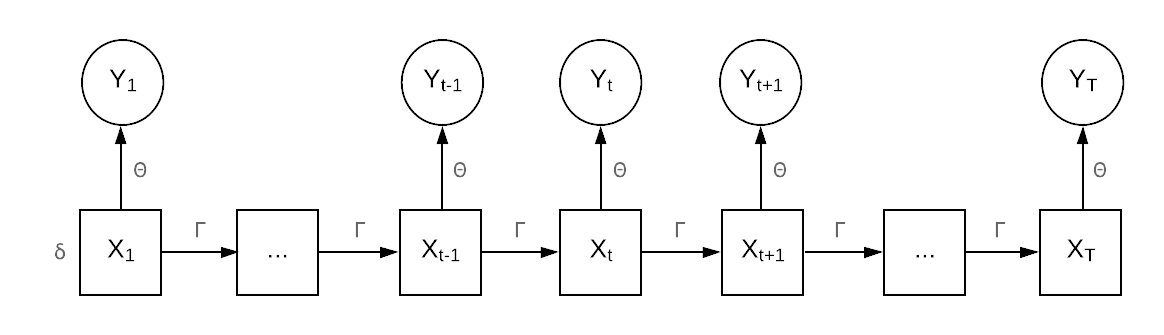
\includegraphics[width=5in]{../Plots/HMM.png}
	\caption{Graphical representation of a traditional HMM.}
	\label{fig:HMM}
\end{figure}


%%%%%%%%%%%%%%%%%%%%%%%%%%%%%%%%%%%%%%%%%
\subsection{The conditionally auto-regressive hidden Markov model (CarHMM)}

One of the key assumptions of an HMM is \textit{conditional independence} between observations, given the state sequence.  Therefore, traditional HMMs do not hold when the observations exhibit certain forms of significant correlation in time.

One way to model extra correlation in an HMM type structure is via a CarHMM, or \textit{conditionally auto-regressive hidden Markov model}, introduced by \citep{Lawler:2019}. Like a traditional HMM, A CarHMM is made up of a Markov chain of unobserved states $X_1,\ldots, X_T$ that can take on values $1, \ldots, N$, with transition probability matrix $\Gamma$ and initial distribution $\delta$ equal to the stationary distribution. Unlike a traditional HMM, the CarHMM assumes that the distribution of the $t$th emission, $Y_t$, conditional on $X_1,\ldots, X_T$ and $ \{Y_1,\ldots, Y_{t-1}\}$, depends on both $X_t$ \textit{and} $Y_{t-1}$. 
The first emission $Y_1$ is assumed to be fixed as an initial value which does not depend upon $X_1$. (Fig \ref{fig:CarHMM}) shows the structure of a CarHMM.

\begin{figure}[ht]
	\centering
	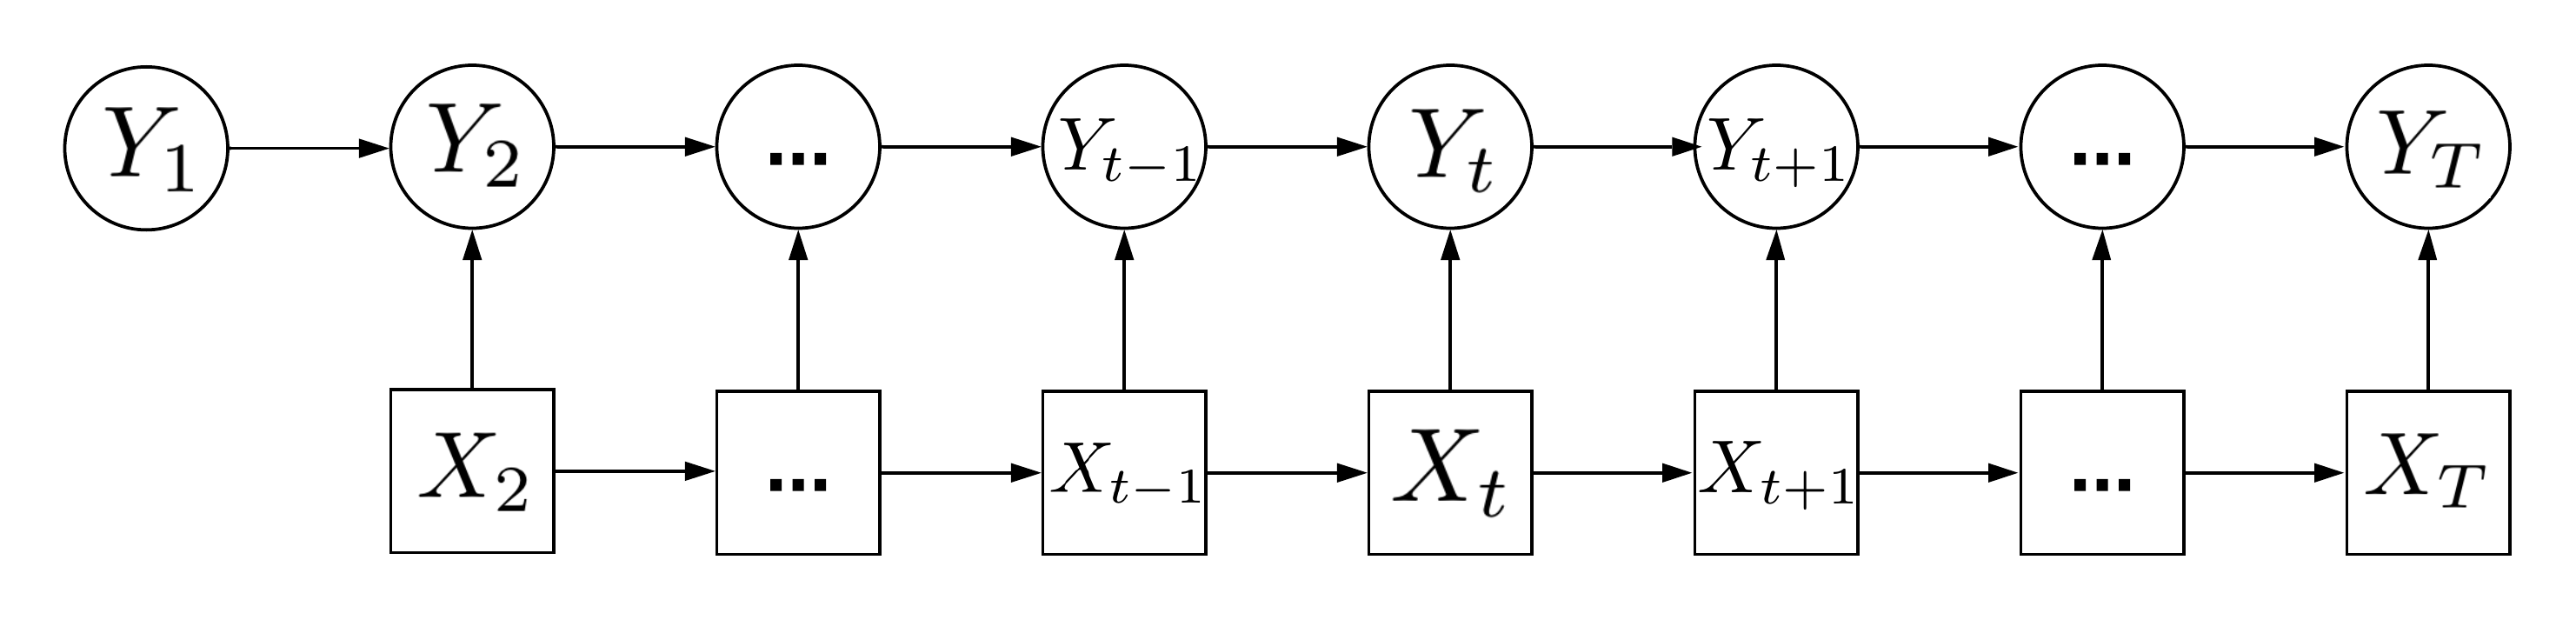
\includegraphics[width=5in]{../Plots/CarHMM.png}
	\caption{Graphical representation of a traditional CarHMM.}
	\label{fig:CarHMM}
\end{figure}

%
We denote the conditional distribution of $Y_t$ given $Y_{t-1}= y_{t-1}$ and $ X_t=i$ as $f^{(i)}( \cdot | y_{t-1})$ or as
$f^{(i)}( \cdot | y_{t-1}; \theta^{(i)})$.
As an example, we could assume that this conditional distribution is normal with parameters $\theta^{(i)} = \{\mu^{(i)},\sigma^{(i)},\phi^{(i)}\}$ where:
%
\[
\mathbb{E}(Y_t|Y_{t-1} = y_{t-1},X_t=i) = \phi^{(i)} ~ y_{t-1} ~+ ~(1-\phi^{(i)})  ~\mu^{(i)}
\]
and
\[
\mathbb{V}(Y_t| Y_{t-1} =y_{t-1}, X_t = i) = (\sigma^{(i)})^2.
\]
%
The CarHMM therefore explicitly models auto-correlation into the emission distributions of the HMM while maintaining the structure needed to write the likelihood using the forward algorithm. In our normal model formulation, we have added only one additional parameter, $\phi^{(i)}$,  per possible hidden state. 

The likelihood for the CarHMM can be easily calculated using the forward algorithm. As previously, let $\bf y$ be the vector of observed emissions. Then
\begin{equation}
\calL_{\text{CarHMM}}(y;\Theta,\Gamma) = \delta \prod_{t=2}^T \Gamma P(y_t|y_{t-1};\Theta) \mathbf{1}_N
\label{CarHMM_likelihood}
\end{equation}
where
%
$P(y_t|y_{t-1};\Theta)$ is an $N \times N$ diagonal matrix with $ii$th entry equal to $f^{(i)}(y_t|y_{t-1}; \theta^{(i)})$.
%

\subsection{The hierarchical hidden Markov model (HHMM)}

A \textit{hierarchical hidden Markov model} contains both a coarse-scale process and a fine-scale process. The coarse-scale process is a hidden Markov model as defined in the previous subsection, with $X_1, \ldots, X_T$ the unobserved Markov chain of states and $Y_1,\ldots, Y_T$ the corresponding observed responses. The possible states are $1,\ldots, N$.   
%
For each value of $t$, the state $X_t$ emits not only $Y_t$ but also a sequence of unobserved states, $X_t^* \equiv (X_{t,1}^*,\ldots, X_{t,T_t^*})$ and a sequence of observed emissions, $Y_t^* \equiv (Y_{t,1}^*,\ldots, Y_{t,T_t^*})$. These form our fine-scale process. The length of each fine-scale process, $T^*_t$, is a problem-specific tuning parameter that is determined by how the fine-scale observations are split. Conditional on the coarse-scale hidden state $X_t$, the joint fine-scale process, $X_t^*$, $Y_t^*$, is a hidden Markov model with parameters depending on the value of $X_t$.  Specifically, given that $X_t=i$, $X_t^*$ is a Markov chain with states $1,\ldots, N_t^*$. The distribution of $X_t^*$, conditional on $X_t=i$, is given by an $N^*_t \times N^*_t$ transition probability matrix $\Gamma^{*(i)}$ and initial probability, denoted by the $N_t^*$-vector $\delta^{*(i)}$, which we take equal to the stationary distribution of the chain. For simplicity, we take $N_t^* \equiv N^*$ although this is not necessary.
%
The distribution of $Y_{t, t^*}$ given $X_{t, t^*}=i^*$ and $X_t=i$ is governed by a parameter $\theta^{(i,i^*)}$, and has density or probability mass function denoted $f^{*(i,i^*)}\left(\cdot; \theta^{(i,i^*)}\right)$ or sometimes simply denoted by $f^{*(i,i^*)}(\cdot)$. Let $\Theta^{*(i)}=\left(\theta^{(i,1)}, \ldots, \theta^{(i,N^*)}\right)$, the fine-scale emission parameter vector corresponding to $X_t=i$.
%
The dependencies among the processes are defined as follows.
%
Given the coarse-scale states, $X_1,\ldots, X_T$, and the coarse scale emissions,  
$Y_1,\ldots, Y_T$, the $T$ fine-scale processes $(X_1^*, Y_1^*), \ldots, (X_T^*, Y_T^*)$, are independent HMMs. It is also possible to force certain parameters to be shared across different coarse or fine states. For example, in our killer whale case study we force certain fine-scale parameters to be shared across coarse-scale hidden states, i.e. $\theta^{(1,i*)} = \ldots = \theta^{(N,i*)}$.

Due to the nested structure of the hierarchical hidden Markov model, the likelihood is easy to calculate via the forward algorithm, just as for HMMs.
%
Let $y$ be the $T$-vector of the observed coarse-scale emissions and
$y^*$ be the $(T_1^* + \cdots T_T^*)$-vector of the observed fine-scale emissions.
%
Let $\Theta^*$ denote the collection of all fine-scale emission parameters,
$\Theta^{*(i)}$, $i=1,\ldots, N$, and let $\Gamma^*$ denote the collection of all fine-scale transition probability matrices, $\Gamma^{*(i)}$, $i=1,\ldots, N$.
%
Then the likelihood of the observed data is:
%
\[
\calL_{\text{HHMM}}(y,y^*;\Theta,\Theta^*,\Gamma,\Gamma^*) = \delta P(y_1,y_1^*;\Theta,\Theta^*,\Gamma^*) \prod_{t=2}^T \Gamma P(y_t,y_t^*;\Theta,\Theta^*,\Gamma^*) \mathbf{1}_N
\]
%
where $P(y_t,y_t^*;\Theta,\Theta^*,\Gamma^*)$ is an $N^ \times N$ diagonal matrix with $ii$th entry corresponding to $X_t=i$ and equal to 
$f^{(i)}(y_t)\calL_{\text{HMM}}\left(y_t^*;\Theta^{*(i)},
\Gamma^{*(i)}\right)$. 

For more information on specific considerations for HHMMs such as incorporating covariates into the probability transition matrix, state decoding, model selection and model checking, see \citep{Adam:2019}.

\begin{figure}[ht]
	\centering
	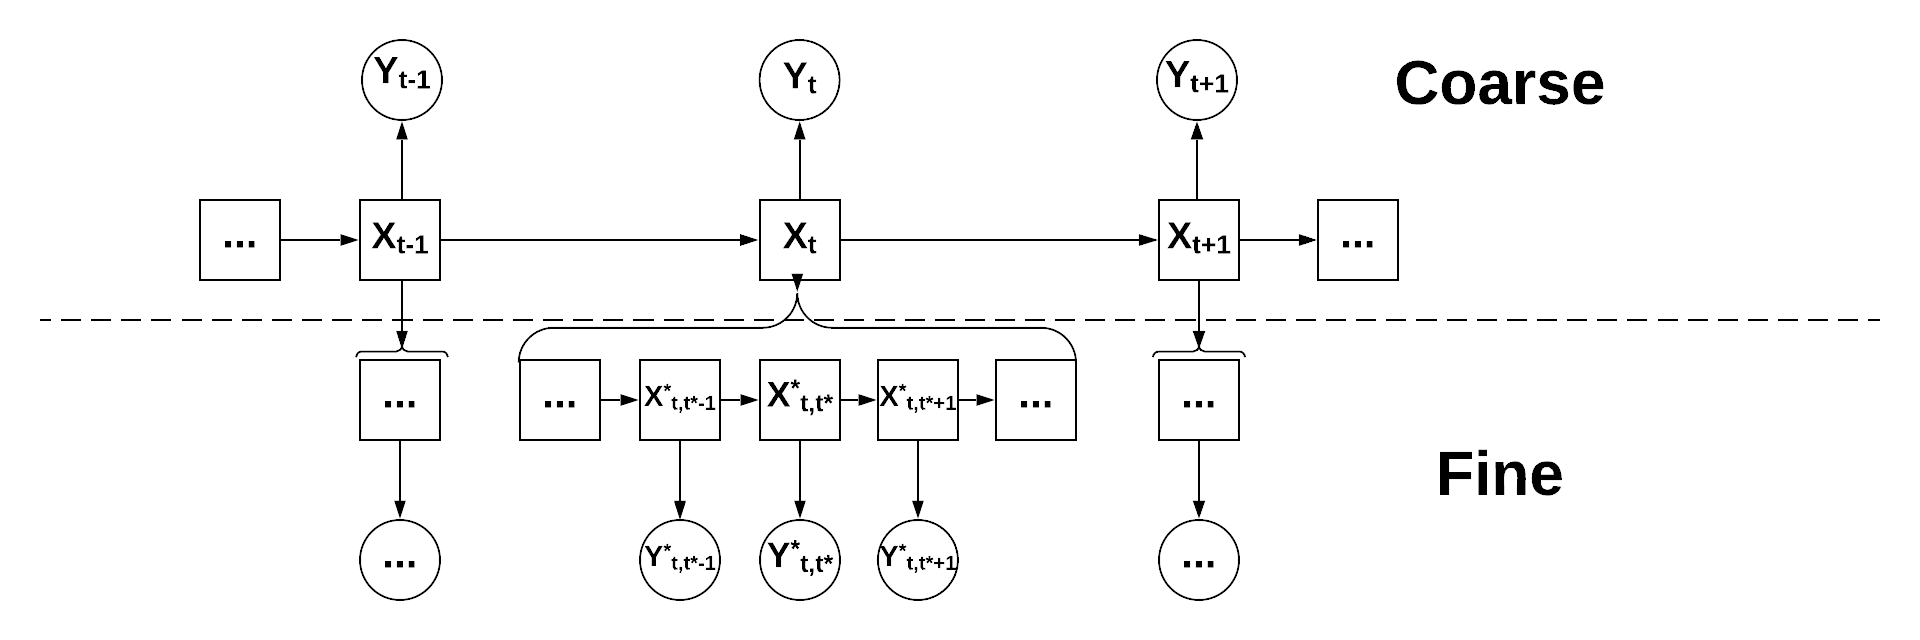
\includegraphics[width=5in]{../Plots/HHMM.png}
	\caption{Graphical representation of a traditional HHMM.}
	\label{fig:HHMM}
\end{figure}



%%%%%%%%%%%%%%%%%%%%%%%%%%%%%%%%%%%%%%%%%
\subsection{General hierarchical structures withing HMMs}
\label{subsec:STFT}

One issue with all HMMs is that they assume Markovian dynamics when conditioned on the hidden state, i.e. that any observation $Y_t$ depends only on the behavioral state $X_t$ and $Y_{t-1}$ when conditioned on all previous time steps. However, there are many processes which violate this Markov property on very fine scales. Using the field of ecology as an example, swimming behaviour of marine mammals often exhibits periodic behavior since the animal repeatedly flukes (swims up and down) to propel itself forward. Work has been done in the past to model non-Markovian dynamics in the \textit{behavioural} process $X^*_t$ \citep{Langrock:2012}, but to our knowledge addressing non-Markovian dynamics within the observation process $Y^*_t$ is still a relatively unstudied area \textcolor{red}{(MAYBE?)}. With improvements in tagging technology allowing for data to be collected at very high frequencies, noisy and non-Markovian fine scale behavior is likely to persist.

To deal with fine-scale structures in the data which violate the Markov property, the fine-scale process $Y^*_t$ can be modeled with \textbf{any} parametric model which admits an easy-to compute likelihood. We remind the reader that the size of each chunk, $T^*_t$, is a problem-specific tuning parameter. It should be long enough to capture the fine-scale behavior within each chunk, but short enough to avoid over-smoothing of the data and to maintain high resolution in the hidden process $X^*$. The state-specific emission distribution $\calL_{\text{HMM}}$ from the HHMM likelihood is then replaced by the likelihood of the fine-scale model, $\calL_{\text{fine}}(\mathbf{y}_t;\Theta^{(i)})$. This gives the following likelihood function:
\[
\calL_{\text{coarse}}(y,y^*;\Theta,\Theta^*,\Gamma) = \delta P(\mathbf{y}_1;\Theta) \prod_{t=2}^T \Gamma P(y,y_t;\Theta,\Theta^*) \mathbf{1}_N
\]
where $P(\mathbf{y}_t;\Theta)$ is an $N \times N$ diagonal matrix with $ii$th entry corresponding to $X_t=i$ and equal to $f^(i)\left(\cdot\right)\calL_{\text{fine}}\left(y^*_t;\Theta^{*(i)}\right)$. This definition is straightforward to extend to the CarHMM on both the coarse- and fine- scale.

We describe one example of a fine-scale model which can simultaneously deal with non-Markovian, periodic behavior and reduce the dimension of the fine-scale process $y^*$.

\subsubsection{The short-time Fourier transform}

Suppose that the fine scale process $y^*_t$ exhibits significant period behavior which cannot be modeled with a Markov chain. One alternative is to use the Fourier transform of $y^*_t$: with a fixed window length $h$:
%
\begin{align*}
    STFT\{z_{(th+1):(th+h)}\}(k) := \hat{z}^{(k)}_{t} = \sum_{n = 1}^{h} z_{(th)+n}e^{-i \frac{2\pi k}{h} (n-1)} \\ k = 0, 1, \ldots, h-1; \quad t = 0,1, \ldots, \lfloor S/h \rfloor - 1
\end{align*}
%
where $i$ in the equation above refers the $\sqrt{-1}$. The STFT slides a moving window of length $h$ across the time series $\mathbf{z}$ and transforms the domain of each window from time to frequency. This allows the spectrum of $\mathbf{z}$ at time $s$ to be summarized by a $h$-dimensional vector of Fourier coefficients. We prevent any overlap in sliding windows to avoid serial dependence. $t$ indexes the \textit{windows} moving across $\mathbf{z}$ while $s$ indexes the \textit{observations} of $\mathbf{z}$. 

If $\mathbf{z} \in \mathbb{R}^{S}$, then $\hat{\mathbf{z}} \in \mathbb{C}^{\lfloor S / h \rfloor \times h}$, which may be very large. Summary statistics can drastically reduce the dimension of $\hat{z}_s$. One possible example is to use the following:
%
$$y_t^{(1)} = \mathcal{R}\left(\hat{z}^{(0)}_t\right) \qquad y_t^{(2)} = \frac{1}{h}\sum_{k=1}^{\tilde{f}}|\hat{z}^{(k)}_s|^2$$
%
$y_t^{(1)}$ is equal to the average value of $\mathbf{z}$ within window $t$, and $y_t^{(2)}$ is equal to the squared 2-norm of the component of $\mathbf{z}$ within the window that can be attributed to frequencies between $1$ and $\tilde{f}$ periods per window length. Like $h$, the max frequency $\tilde{f}$ is a problem-specific tuning parameter. It should be selected such that $\tilde{f}$ periods per window length is the maximum frequency of $\mathbf{z}$ that makes biological sense. These summary statistics are just one possible choice to describe each window; other choices include the maximum and argmax of $\hat z_t$. Figure (\ref{fig:fourier_example}) visually shows the process of moving from $\mathbf{z}$ to $\mathbf{y}$.

\begin{figure}[ht]
	\centering
	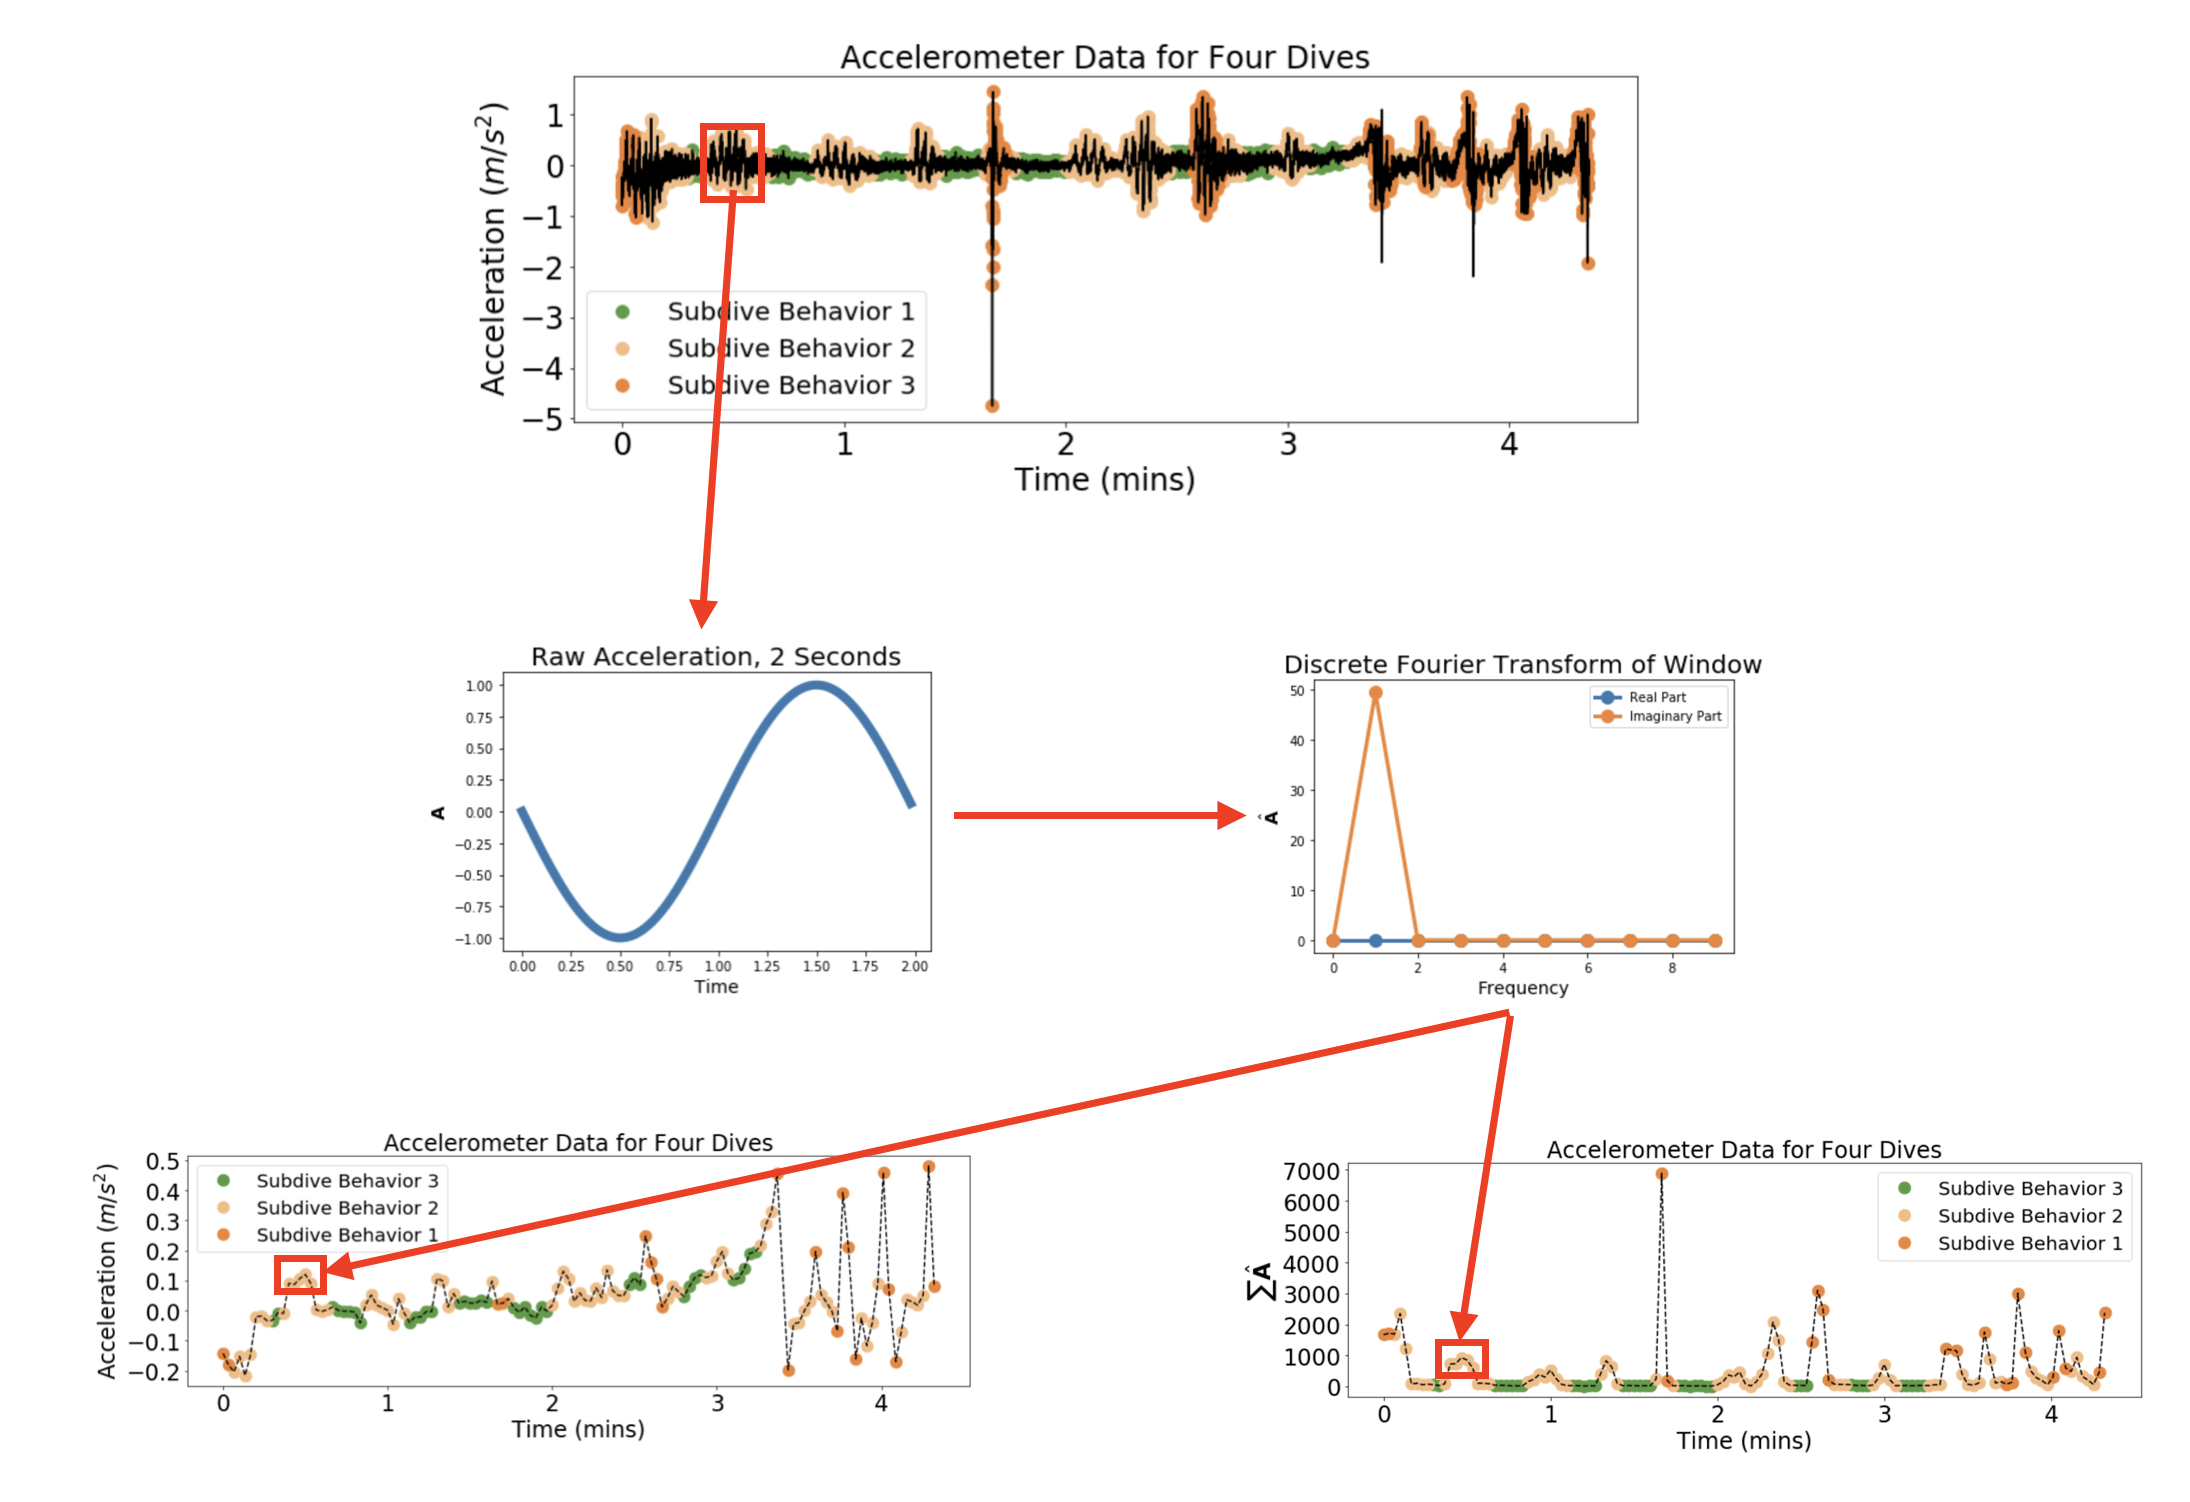
\includegraphics[width=5in]{../Plots/fourier_transform.png}
	\caption{Visualization of transforming $\mathbf{z}_t$ into $\mathbf{y}_t$ using a sliding window and Fourier transform.}
	\label{fig:fourier_example}
\end{figure}

It is possible to accommodate for unequal time steps within each window by using the \textbf{non-uniform discrete Fourier transform (NDFT)}. We do not describe the details of this method in this work, but the generalization is straightforward. Refer to Bagchi et al \citep{Bagchi:1999} for details.

